%===================================================================================
% Chapter: Metodologia
%===================================================================================
\chapter{Experimentación y Resultados}\label{chapter:resultados}
%\addcontentsline{toc}{chapter}{Marco Teórico}
%===================================================================================

En este cápitulo bla bla

\section{Datos para la Validación del Modelo}
En el presente trabajo los datos provienen del Estudio en Lactantes Fase I/II para PCV7-TT (Instituto Finlay de Vacunas, 2019) 

\section{Metaheurística para la Exploración del Espacio de Parámetros}
Aquí se presenta la metaheurística empleada para la optimización de los parámetros del modelo. Se explica su funcionamiento, configuración y justificación de su elección.

% Ejemplo:
% Se utilizó un algoritmo genético con población de tamaño [n], tasa de mutación de [x], y número máximo de iteraciones [y].

\section{Métrica de Optimización}
Se define la métrica utilizada como función objetivo durante el entrenamiento del modelo, explicando su relevancia y método de cálculo.

% Ejemplo:
% La métrica optimizada fue el error cuadrático medio (MSE) entre las salidas simuladas y los datos reales, calculado como...

\section{Proceso de Validación con el Grupo de Test}
Se detalla cómo se realizó la validación final del modelo utilizando un conjunto de test independiente, incluyendo metodología, resultados obtenidos y análisis.

% Ejemplo:
% El conjunto de test consistió en [descripción]. Los resultados muestran que el modelo alcanzó un [valor] en la métrica MSE, indicando...

\section{Discusión de Resultados}
Se analizan los resultados obtenidos, su significado, comparación con trabajos previos y posibles limitaciones.

% Aquí puedes incluir tablas, figuras y análisis estadísticos relevantes.






% \begin{figure}[h] % h = here (aquí)
%     \centering
%     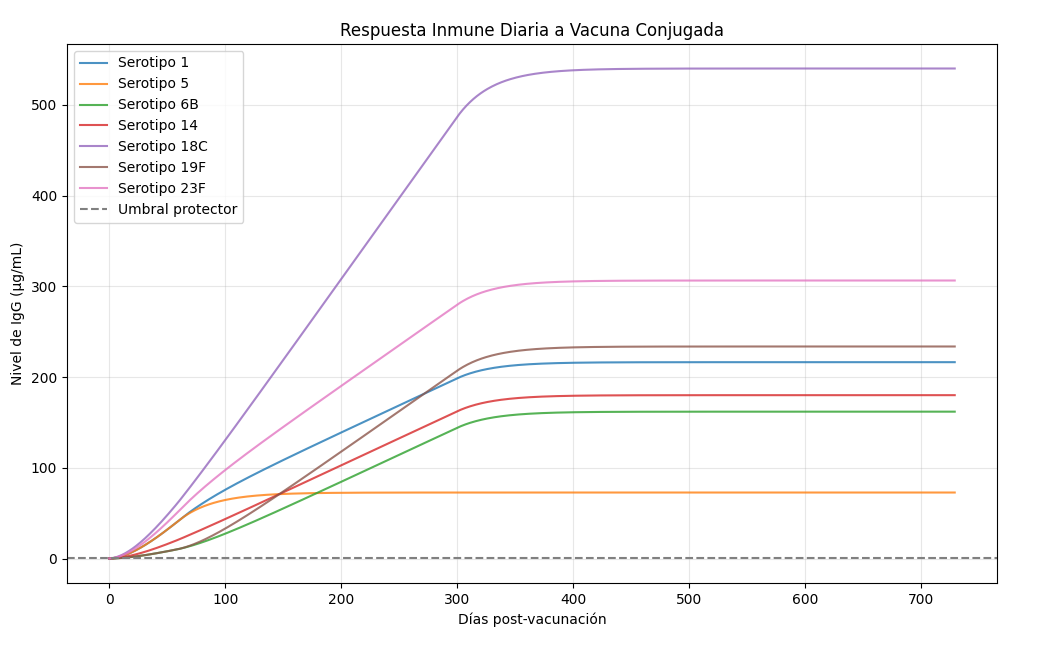
\includegraphics[width=1\textwidth]{Graphics/res.png}
%     \caption{a}
%     \label{fig:etiqueta}
% \end{figure}

% \begin{figure}[h] % h = here (aquí)
%     \centering
%     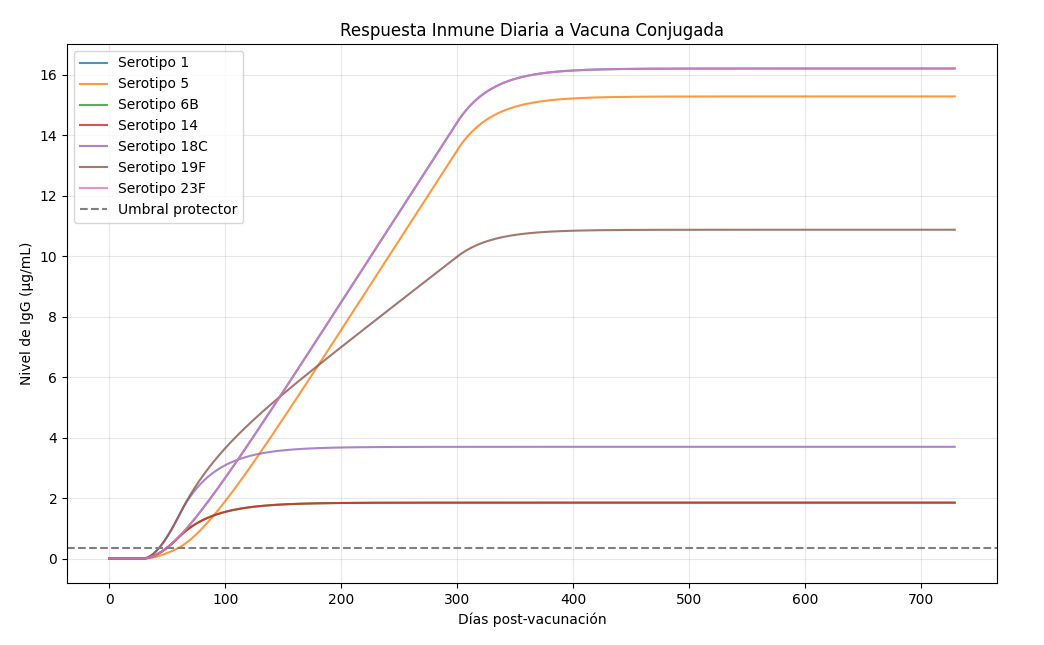
\includegraphics[width=1\textwidth]{Graphics/res1.png}
%     \caption{a}
%     \label{fig:etiqueta}
% \end{figure}

% \begin{figure}[h] % h = here (aquí)
%     \centering
%     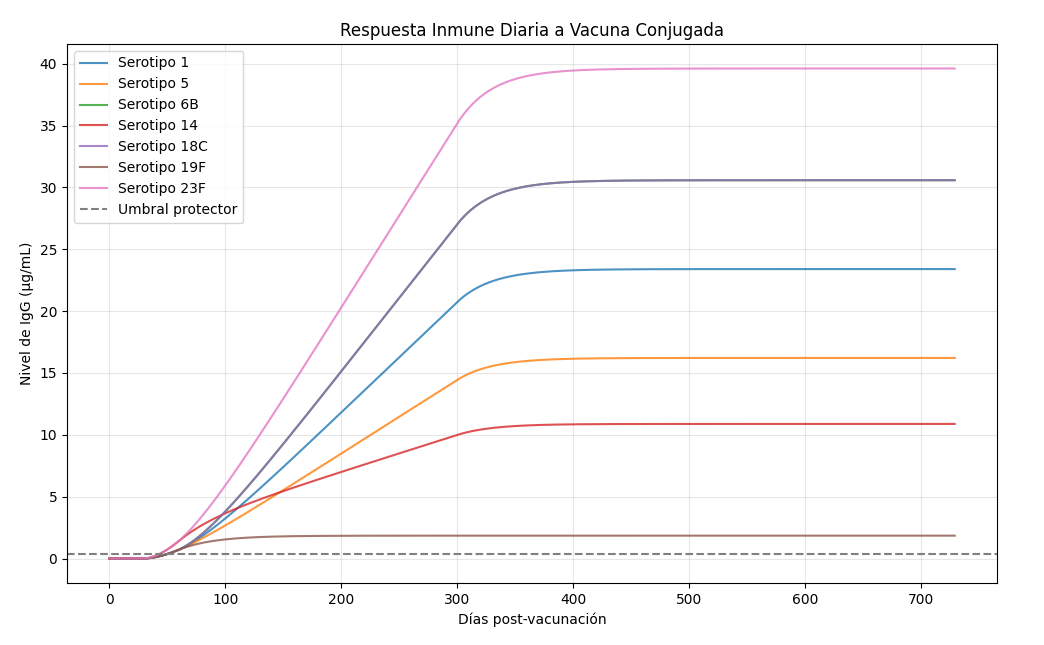
\includegraphics[width=1\textwidth]{Graphics/res2.png}
%     \caption{a}
%     \label{fig:etiqueta}
% \end{figure}

% \begin{figure}[h] % h = here (aquí)
%     \centering
%     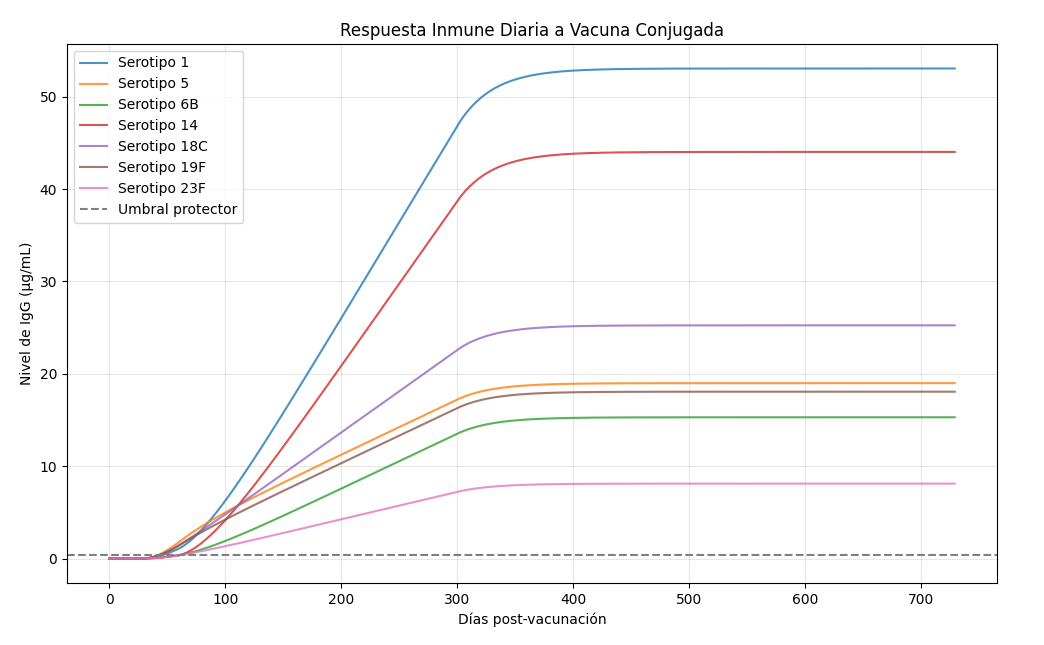
\includegraphics[width=1\textwidth]{Graphics/res3.png}
%     \caption{a}
%     \label{fig:etiqueta}
% \end{figure}